\documentclass[12pt, letterpaper]{report}
%\usepackage[mtbold]{mathtime}
\usepackage{enumerate}
\usepackage{xypic}

\setlength{\oddsidemargin}{0in}
\setlength{\evensidemargin}{0in}
\setlength{\textwidth}{6.5in}
\setlength{\topmargin}{0in}
\setlength{\textheight}{8.5in}

\setcounter{topnumber}{3}%
\def\topfraction{.7}%
\setcounter{bottomnumber}{1}
\def\bottomfraction{.3}
\setcounter{totalnumber}{5}%
\def\textfraction{.1}% was .2
\def\floatpagefraction{.7}% was .7
\setcounter{dbltopnumber}{2}
\def\dbltopfraction{.7}
\def\dblfloatpagefraction{.5}
%\addtolength{\parskip}{\baselineskip}

\long\def\comment#1{\ignorespaces}

\pagestyle{myheadings}

%% Parameters to the \lecture command are the lecture number, the
%% date, and the scribe's name.
\newcommand{\lecture}[3]{\newpage\markboth{\textit{Lecture #1, #2}}{\textit{Lecture #1, #2}}
{
\begin{flushleft}
\LARGE{\bf Lecture #1}\\
\LARGE{\bf #2}\\
\end{flushleft}}
\bigskip}

\newenvironment{example}{\begin{quote}}{\end{quote}}
\newenvironment{letter}[1]{\begin{enumerate}[a.]\item[#1.]}{\end{enumerate}}
\newenvironment{letters}{\begin{enumerate}[a.]}{\end{enumerate}}
\newcommand{\xmp}[1]{\textit{#1}}
\newcommand{\good}{\emph{Good:}}
\newcommand{\bad}{\emph{Bad:}}
\newcommand{\ok}{\emph{OK:}}
\newcommand{\better}{\emph{Better:}}
\newcommand{\wrong}{\emph{Wrong:}}
\newcommand{\correct}{\emph{Right:}}

\newtheorem{theorem}{Theorem}
\newtheorem{lemma}[theorem]{Lemma}
\newtheorem{corollary}[theorem]{Corollary}

% Make captions with bold figure/table name and number.
\makeatletter
\long\def\@makecaption#1#2{%
  \vskip\abovecaptionskip
  \sbox\@tempboxa{\small\textbf{#1:} #2}%
  \ifdim \wd\@tempboxa >\hsize
    {\small\textbf{#1:} #2}\par
  \else
    \global \@minipagefalse
    \hb@xt@\hsize{\hfil\box\@tempboxa\hfil}%
  \fi
  \vskip\belowcaptionskip}
\makeatother

\newcommand{\figcaption}[1]{\caption[]{#1}}
\newcommand{\figpart}[1]{\textbf{(#1)}~\ignorespaces}

\newcommand{\subheading}[1]{\subsubsection*{#1}}
\newcommand{\subsubheading}[1]{\paragraph*{#1.}}

\newcommand{\defn}[1]{\emph{#1}}

\newcommand{\eqnref}[1]{(\ref{#1})}
\renewcommand{\cases}[1]{\left\{ \begin{array}{ll}#1\end{array}\right.}
\newcommand{\cif}[1]{\mbox{if $#1$}}

\newcommand{\prob}[1]{\Pr\left\{ #1 \right\}}
\renewcommand{\hat}{\widehat}
\newcommand{\elems}[3]{#1, \lb #2, \lb \ldots, #3}
\renewcommand{\vector}[1]{(#1)}
\newcommand{\evector}[3]{\vector{\elems{#1}{#2}{#3}}}
\newcommand{\seq}[1]{\langle#1\rangle}
\newcommand{\set}[1]{\{#1\}}
\newcommand{\eset}[3]{\set{\elems{#1}{#2}{#3}}}
\def\ceil#1{\left\lceil#1\right\rceil}
\def\floor#1{\left\lfloor#1\right\rfloor}
\newcommand{\abs}[1]{\left|#1\right|}
\newcommand{\card}[1]{\left|#1\right|}
\newcommand{\smallcard}[1]{|#1|}
\newcommand{\proof}{\noindent\textit{Proof:}\hspace*{1em}}
\newcommand{\proofof}[1]{\noindent\textit{Proof of #1:}\hspace*{1em}}
\newcommand{\proofsketch}{\noindent\textit{Proof sketch:}\hspace*{1em}}
\newcommand{\proofnote}[1]{\noindent\textit{Proof:}\hspace*{.1em}\footnote{#1}\hspace*{0.5em}}
\def\twodots{\mathinner{\ldotp\ldotp}}
\newcommand{\range}{\twodots}
\newcommand{\inv}{^{-1}}
\newcommand{\transpose}{^{\rm T}}
\newcommand{\ptranspose}{^{\prime{\rm T}}}
\newcommand{\oneone}{\stackrel{\mbox{\scriptsize 1-1}}{\rightarrow}}
\newcommand{\xor}{\oplus}
\newcommand{\bigxor}{\bigoplus}
\def\degrees{^{\circ}}

\DeclareMathSymbol{\umod}{\mathbin}{operators}{"23}

\def\qedbox{\hspace{-0.3em}\mbox{\vrule height 5pt width 5pt}}
\def\qed{\unskip\parfillskip=0pt~~~~\hfill\llap{\vrule height 5pt width 5pt}\vskip11pt\parfillskip=0pt plus 1fil\relax}
\def\qednoproof{\unskip\parfillskip=0pt~~~~\hfill\llap{\vrule height 5pt width 5pt}}

\newenvironment{eqnarrayreason}{\[\begin{array}{rcll}}{\end{array}\]}
\newcommand{\eqnline}{\\[.75ex]}
\newcommand{\bigeqnline}{\\[2.5ex]}

\newlength{\savearraycolsep}
\newcommand{\narrowarray}[1]{\setlength{\savearraycolsep}{\arraycolsep}%
\setlength{\arraycolsep}{#1\arraycolsep}}
\newcommand{\normalarray}{\setlength{\arraycolsep}{\savearraycolsep}}
\newlength{\savetabcolsep}
\newcommand{\narrowtabular}[1]{\setlength{\savetabcolsep}{\tabcolsep}%
\setlength{\tabcolsep}{#1\tabcolsep}}
\newcommand{\normaltabular}{\setlength{\tabcolsep}{\savetabcolsep}}

\newcommand{\noarraystretch}{\def\arraystretch{}}
\newcommand{\matx}[2]{{\noarraystretch\left[\begin{array}{*{#1}{c}}#2\end{array}\right]}}
\newcommand{\block}[2]{{\noarraystretch\count200=#1%
\advance\count200 by -1\left[\begin{array}{*{\count200}{c|}c}#2\end{array}\right]}}
\newcommand{\hatstrut}{\rule{0pt}{3ex}}

\newcommand{\bstrut}{\rule{0pt}{2.4ex}}
\newcommand{\bline}{\hline\bstrut}
\newlength{\blockdimwidth}
\newcommand{\bm}[1]{\makebox[\blockdimwidth]{$#1$}}
\newcommand{\bt}[1]{\makebox[\blockdimwidth]{\footnotesize$#1$}}
\newcommand{\bs}[1]{\mbox{\bstrut\footnotesize$#1$}}
\newcommand{\blockdims}[6]{{\noarraystretch\setlength{\blockdimwidth}{#1}%
\begin{array}{cc@{\hspace{0em}}c} &%
\begin{array}{c*{#2}{c}}#4\end{array} & \\%
#3 &
\count200=#2\advance\count200 by -1%
\left[\begin{array}{*{\count200}{c|}c}#5\end{array}\right] &%
\begin{array}{l}#6\end{array}%
\end{array}}}
\newcommand{\blockdimscol}[6]{{\noarraystretch\setlength{\blockdimwidth}{#1}%
\begin{array}{cc@{\hspace{0em}}c} &%
\begin{array}{cc}#4\end{array} & \\%
#3 &
\left[\begin{array}{c}#5\end{array}\right] &%
\begin{array}{l}#6\end{array}%
\end{array}}}
\newcommand{\blockdimstoponly}[5]{{\noarraystretch\setlength{\blockdimwidth}{#1}%
\begin{array}{cc} &%
\begin{array}{c*{#2}{c}}#4\end{array}\\%
#3 &
\count200=#2\advance\count200 by -1%
\left[\begin{array}{*{\count200}{c|}c}#5\end{array}\right]%
\end{array}}}
\newcommand{\blockdimsmatxonly}[5]{{\noarraystretch\setlength{\blockdimwidth}{#1}%
\begin{array}{c@{\hspace{0em}}c}%
\begin{array}{c*{#2}{c}}#3\end{array} & \\%
\count200=#2\advance\count200 by -1%
\left[\begin{array}{*{\count200}{c|}c}#4\end{array}\right] &%
\begin{array}{l}#5\end{array}%
\end{array}}}
\newcommand{\blockdimstopmatxonly}[4]{{\noarraystretch\setlength{\blockdimwidth}{#1}%
\begin{array}{c@{\hspace{0em}}c}%
\begin{array}{c*{#2}{c}}#3\end{array} & \\%
\count200=#2\advance\count200 by -1%
\left[\begin{array}{*{\count200}{c|}c}#4\end{array}\right]%
\end{array}}}

\usepackage{url}
\urlstyle{rm}

\usepackage{epsfig,graphicx,epsf,subfigure, amssymb,amsmath}
\usepackage{amssymb,amsmath,subfigure}
%\usepackage{graphics}
\usepackage{setspace}
\def\doublespace{\doublespacing}
\usepackage{booktabs}
\usepackage{caption}

\usepackage{fancyheadings}
\usepackage{epsfig}
%\usepackage{amssymb,amsmath}
%\usepackage{a4 wide}
\usepackage{algorithmic}
\usepackage{algorithm}
\usepackage{rotating}
\usepackage{hyperref}

\usepackage{amsfonts,latexsym}
%\usepackage[amsthm,thmmarks,thref]{ntheorem}
%\usepackage{accents} % To produce symbols for definitions etc.
\usepackage{epsf}

\setlength{\oddsidemargin}{0in} \setlength{\evensidemargin}{0in}
\setlength{\textwidth}{6.5in} \setlength{\topmargin}{0in}
\setlength{\textheight}{8.5in}

\long\def\gobble#1{}
\def\cref#1{#1}
\usepackage{boxedminipage}
%\def\codesize{\scriptsize}
\def\codesize{\footnotesize}
\newcommand{\capspacing}{\footnotesize}
\def\rulefigure{\smallskip\hrule}

\renewcommand{\bibname}{References}
\newcommand{\Omit}[1]{}
% ~~~~~~~ page style setting for main part ~~~~~~~
\addtolength{\headheight}{3pt} \pagestyle{fancy}
\setlength{\headrulewidth}{0.1pt}
\renewcommand{\chaptermark}[1]{\markboth{\chaptername\ \thechapter. #1}{}}
\lhead{\fancyplain{}{\bfseries\footnotesize\sc\leftmark}} \rhead{}
\addtolength{\headsep}{-0.1in}
\cfoot{\fancyplain{}{\bfseries\rm\thepage}}

%from LectureTony:
\font\sletter=msbm10
\def\Rsmall{\mbox{\sletter R}}
\def\Real{\Rsmall}

\def\figcredit#1{Credit: {#1}}

%\setlength{\oddsidemargin}{0.5cm}\setlength{\evensidemargin}{0.5cm}

\begin{document}
\doublespacing
\bibliographystyle{plain}

\title{\textbf{Final Project: Computational Design of Binding Peptide Using Dead-End Elimination}\\[2em]}


\author{\textbf{Ari J. Willig} \\[1em]}


\date{\textbf{2026}}
\maketitle \thispagestyle{empty}
\newpage

\pagenumbering{roman}

\include{ack}
\include{insert}
{\small\tableofcontents}
\newpage
\pagenumbering {arabic}
\newtheorem{ex}{Example}
\newtheorem{dfn}{Definition}
\newtheorem{probl}{Problem}
\newcommand{\bx}{{\bf x}}

 \setcounter{chapter}{1} \def\AS{{$A^*$}}

\section{Abstract}
Protein–protein interactions (PPIs) underlie most biological processes, and many therapeutic strategies aim to modulate these interactions to achieve clinical outcomes. Computational peptide design offers a way to engineer such interactions with high specificity while minimizing experimental workload. In this project, a peptide was computationally designed targeting the MDM2 hydrophobic pocket using Dead-End Elimination (DEE) \cite{Dahiyat}, a combinatorial optimization algorithm for rotamer selection. Starting from the backbone conformation of the native p53 transactivation domain peptide from PDB structure 1YCR \cite{PDB}, side-chain identities and conformations at three variable positions were optimized using a simplified pairwise energy function accounting for van der Waals interactions and hydrophobic burial. DEE pruned 94 of 102 total rotamers across three design positions, reducing the search space by 99.97\% before exhaustive enumeration identified the global minimum energy sequence LEU-VAL-VAL, replacing the native THR-SER-LEU. The designed peptide scored more favorably than the native p53 binder when evaluated on the simplified scoring function, due to hydrophobic substitutions. However, validation using the Rosetta ref2015 energy function \cite{RosettaScoring} revealed the native structure to be more stable, highlighting the limitations of simplified scoring functions and motivating the use of more physically complete energy models in future experiments. The code used in this study is available at \href{https://git@github.com:Ari-Willig/CS590FinalProject.git}{this GitHub repository}

\section{Introduction}
Protein-protein interactions (PPIs) govern a vast array of biological processes, and their central role in disease has made them attractive targets for therapeutic intervention. Yet designing molecules that disrupt or modify these interactions with high specificity remains extremely challenging.

\begin{figure}[h]
\centering
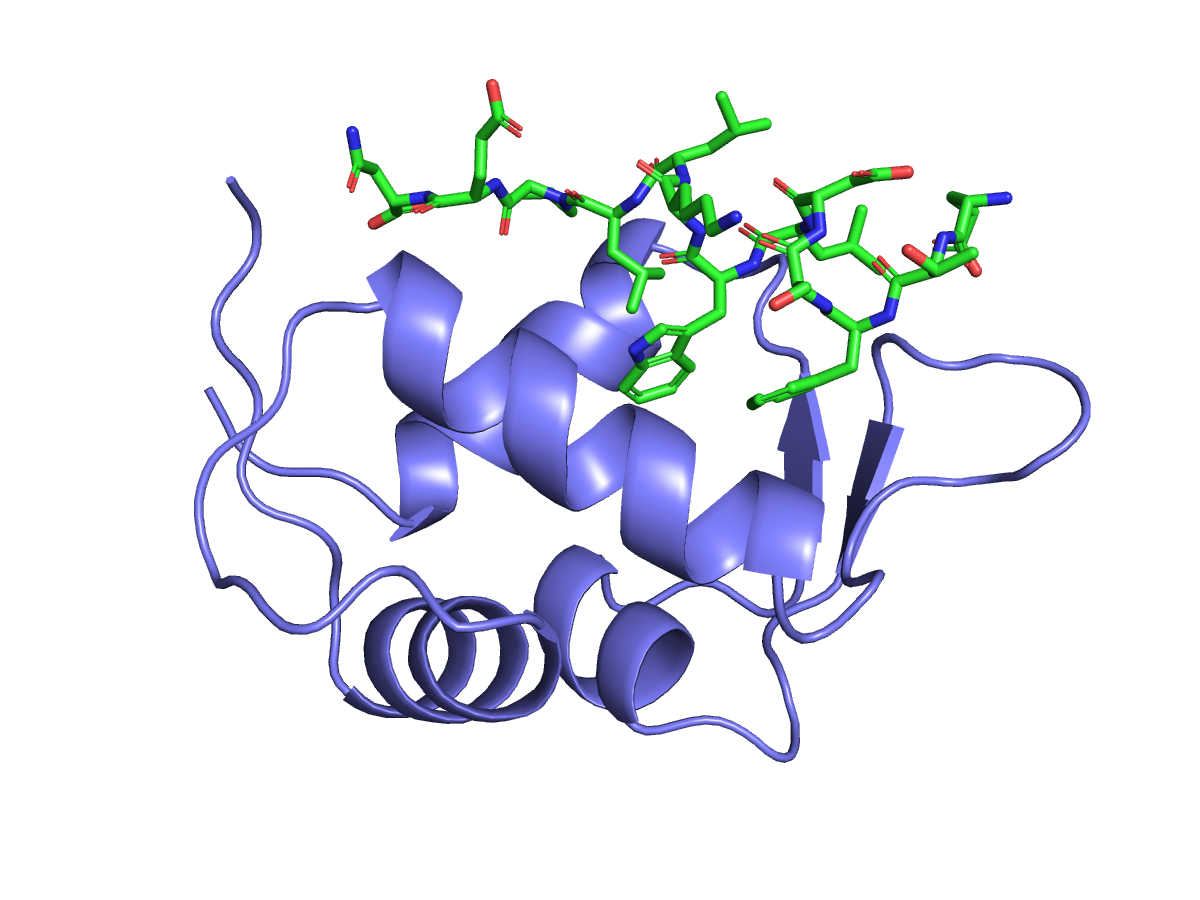
\includegraphics[width=6in]{MDM2p53_figure1_nowatermarkpng.png}
\caption{PyMOL representation of the MDM2-p53 binding interaction. MDM2 represented as a ribbon diagram and p53 represented as a stick model.
\figcredit{Ref.~\cite{PyMOL}.}} 
\label{fig:seq_result}
\end{figure}

One well-studied example is the interaction between the E3 ubiquitin ligase MDM2 and the tumor suppressor protein p53, shown in Figure \ref{fig:seq_result}. MDM2 binds the N-terminal transactivation domain of p53 and targets it for proteasomal degradation, effectively suppressing p53-mediated apoptosis and cell cycle arrest. Because MDM2 overexpression is observed across many human cancers, this interaction has emerged as an important therapeutic target \cite{NCBI}. The binding interface is well characterized, and high-resolution structural data for the MDM2–p53 complex is available from the Protein Data Bank \cite{PDB}, making it an ideal model system for computational peptide design.

Most computational approaches to peptide design seek to identify amino acid sequences that optimize predicted binding affinity to a target structure. The central challenge is combinatorial: the enormous number of possible sequence and rotamer combinations causes the search space to grow exponentially with peptide length. Dead-End Elimination (DEE) addresses this by provably pruning rotamer configurations that cannot belong to the global minimum energy conformation (GMEC), substantially reducing the conformational search without sacrificing optimality guarantees.

Modern protein design algorithms, while powerful, often demand substantial expertise, specialized infrastructure, and computational resources that place them out of reach for many researchers and students. This project explores whether meaningful peptide design is possible using more tractable methods. We implement a streamlined version of DEE to design a binding peptide targeting the MDM2–p53 interface, prioritizing accessibility and interpretability over the full complexity of state-of-the-art pipelines. The MDM2–p53 system was chosen to evaluate this simplified framework because it is so well characterized, providing a meaningful benchmark for what can be achieved under significant simplifying assumptions.

\section{Overview of Methodology}
Given the coordinates of the MDM2-p53 complex \cite{PDB}, the pipeline developed in this project (1) identifies the MDM2 binding pocket geometrically by selecting residues within 8 Angstroms of the native p53 peptide, (2) optimizes side-chain identity and conformation at three variable peptide positions using a simplified pairwise energy function consisting of van der Waals and hydrophobic burial terms (3) applies the Goldstein DEE criterion \cite{Dahiyat} to provably prune rotamer configurations incompatible with the global minimum energy conformation, and (4) identifies the optimal sequence by exhaustive enumeration over the pruned rotamer search space. The designed peptide was then compared against the native p53 peptide using both the simplified scoring function and the Rosetta ref2015 energy function \cite{RosettaScoring} as a validation of design quality. Structural comparison of the designed binder and the native peptide was then performed using PyMOL \cite{PyMOL}.

\subsection{Pocket Identification and Peptide Residue Extraction}
Prior to peptide optimization, the MDM2-p53 binding interface was characterized from the coordinates of PDB structure 1YCR. MDM2 and p53 residues were extracted from chains A and B respectively, and binding pocket residues were defined as all MDM2 residues containing at least one atom within 8 Angstroms of any p53 atom. Heteroatoms and crystallographic water molecules were excluded from this definition, as they are not part of the native protein structure. The p53 peptide backbone was treated as rigid throughout all subsequent steps, with new side chain conformations computed relative to the fixed backbone coordinates extracted from the crystal structure.

\subsection{Rotamer Library Construction}
The rotamer library was constructed from the top three most probable conformations per amino acid as reported in the Penultimate Rotamer Library \cite{rotamerlib}. Amino acid types were selected based on their frequency of appearance in the MDM2 binding pocket, hydrophobic character consistent with the pocket environment, and chemical diversity. Chi angles were set to the modal values reported for each rotamer bin. Restricting the library to a small set of conformations per amino acid kept the rotamer search space computationally tractable while preserving the most relevant side-chain geometries.

\subsection{Energy Function}
The energy function used in this pipeline is defined by the approach in \cite{Dahiyat} using the Goldstein criterion. The total energy of a given rotamer assignment is expressed as a pairwise additive function:

\begin{equation}
E_{\text{total}} = \sum_{i} E_{\text{self}}(i, r_i) + \sum_{i < j} 
E_{\text{pair}}(i, r_i, j, r_j)
\label{eq:total_energy}
\end{equation}

\noindent where $i$ and $j$ index the design positions, and $r_i$ and $r_j$ denote the rotamer assigned at each position. The self energy represents the interaction between a single rotamer and the fixed MDM2 binding pocket, and is defined as:

\begin{equation}
E_{\text{self}}(i, r_i) = \sum_{k \in \text{pocket}} E_{\text{vdW}}(d_{ik}) 
+ E_{\text{hydrophobic}}(i, r_i)
\label{eq:self_energy}
\end{equation}

\noindent where $d_{ik}$ is the distance between the side chain centroid of rotamer $r_i$ and the centroid of pocket residue $k$. The van der Waals interaction is modeled using a soft Lennard-Jones potential \cite{vdw_energy}:

\begin{equation}
E_{\text{vdW}}(d) = 
\begin{cases} 
100 & \text{if } d < 1.0 \text{ \AA} \\
\min\left(\epsilon \left[\left(\dfrac{r_{\min}}{d}\right)^{12} - 
2\left(\dfrac{r_{\min}}{d}\right)^{6}\right],\ 100\right) & \text{otherwise}
\end{cases}
\label{eq:vdw}
\end{equation}

\noindent where  $\epsilon = 1$, $r_{\min} = 3.5$ \AA\ is the distance at the energy minimum, and the repulsive term is capped at 100 to prevent extreme variation at short distances.

\begin{figure}[H]
\centering
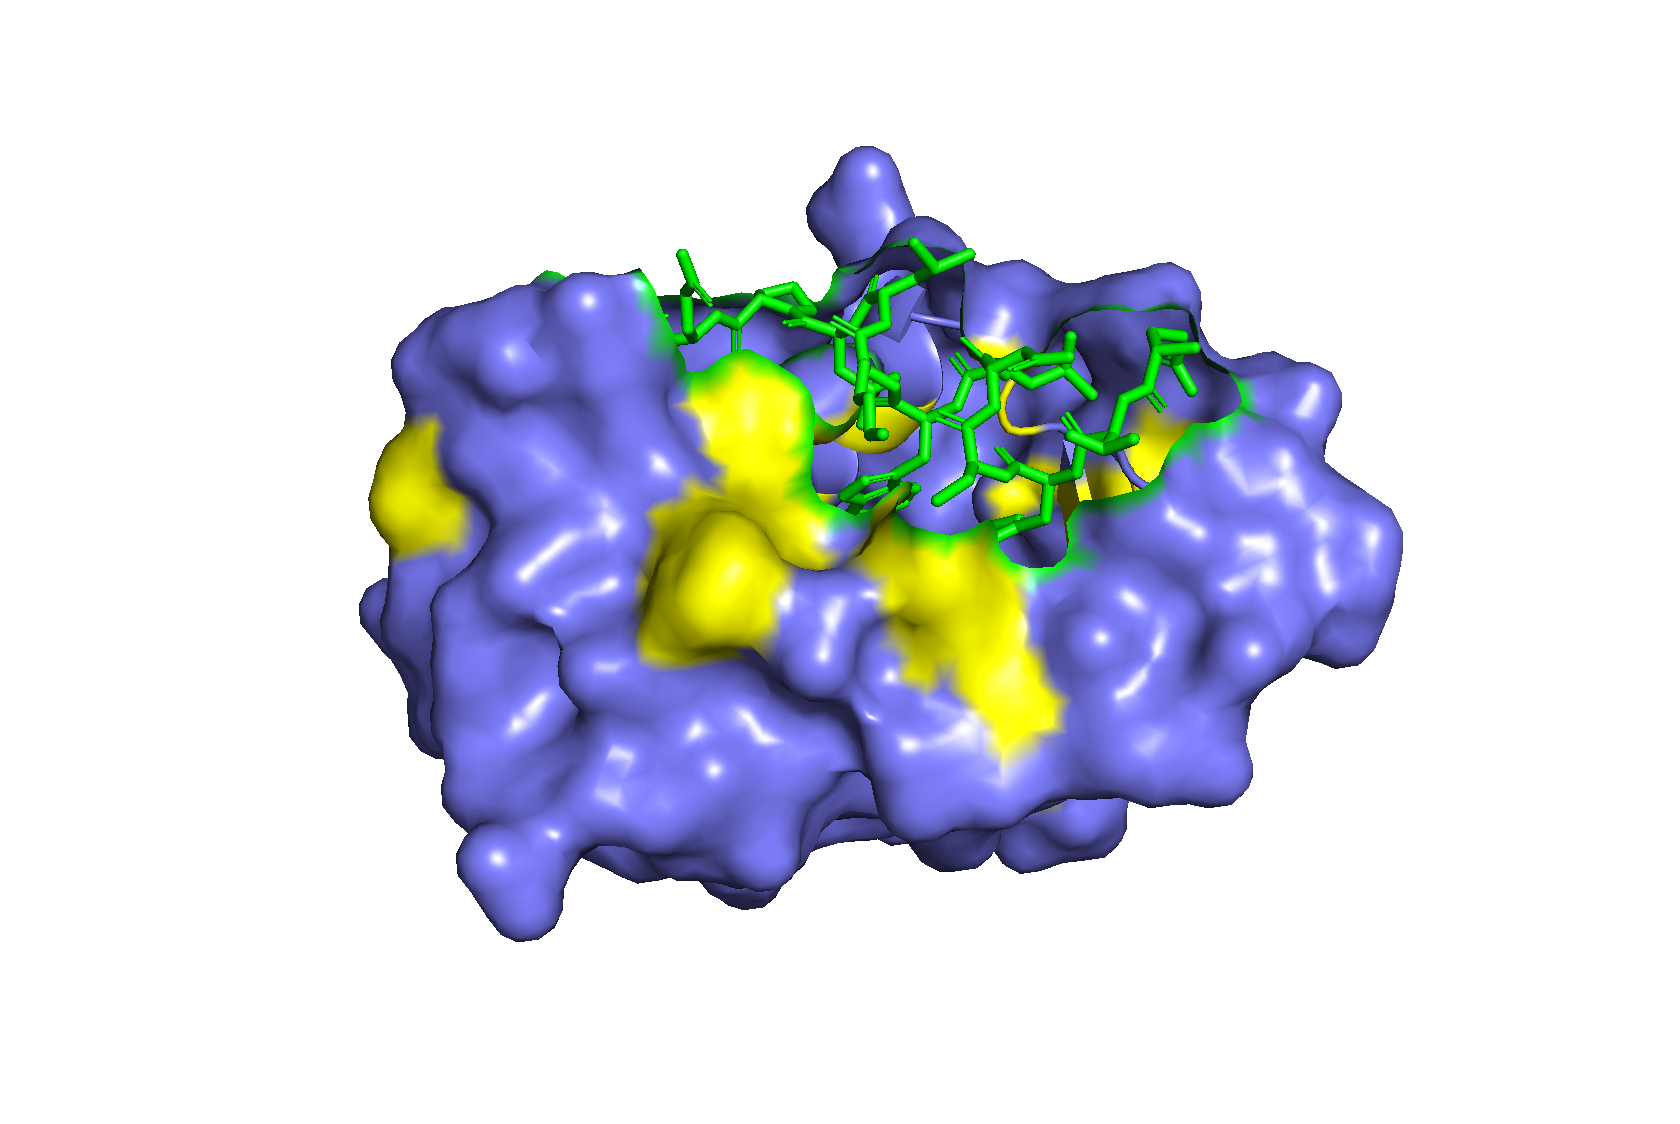
\includegraphics[width=6in]{MDM2p53_hydrophobicity.png}
\caption{PyMOL representation showing the surface of the MDM2 ubiquitin ligase and the p53 tumor suppressor in its binding pocket. The yellow coloring on the MDM2 surface represents hydrophobic residues.
\figcredit{Ref.~\cite{PyMOL}.}}
\label{fig:hydrophobicity}
\end{figure}

The self energy also includes a hydrophobic burial term due to the hydrophobic nature of the MDM2 binding pocket, shown in Figure \ref{fig:hydrophobicity}. This term rewards hydrophobic residues for pocket contacts and penalizes polar residues:

\begin{equation}
E_{\text{hydrophobic}}(i, r_i) = 
\begin{cases}
-0.5 \times n_{\text{contacts}} & \text{if } r_i \text{ is hydrophobic} \\
+0.3 \times n_{\text{contacts}} & \text{otherwise}
\end{cases}
\label{eq:hydrophobic}
\end{equation}

\noindent where $n_{\text{contacts}}$ is the number of pocket residue centroids within 5.0 \AA\ of the side chain centroid of rotamer $r_i$. The pairwise interaction energy between two peptide rotamers at design positions $i$ and $j$ is modeled purely as a van der Waals interaction between side chain centroids:

\begin{equation}
E_{\text{pair}}(i, r_i, j, r_j) = E_{\text{vdW}}(d_{ij})
\label{eq:pair_energy}
\end{equation}

\noindent where $d_{ij}$ is the distance between the side chain centroids of rotamers $r_i$ and $r_j$.

Several simplifications were made to keep the energy function computationally tractable and within the scope of this study. First, side chain positions were represented by a single centroid coordinate rather than full atomic coordinates, reducing the cost of distance calculations while preserving the geometry of pocket interactions. Second, explicit electrostatic interactions were omitted because of the predominantly hydrophobic character of the MDM2 binding pocket, where van der Waals and burial terms are expected to dominate. Third, no backbone energy term was included, as the peptide backbone was treated as fully rigid throughout the design process, making its contribution to the total energy constant and therefore irrelevant to optimization. Finally, conformational entropy was neglected, consistent with the simplified scope of this work.

All self and pair energies were computed and stored in lookup tables prior to DEE implementation so that repeated access of these values was more efficient.

\subsection{Dead-End Elimination}
The computational tractability of this pipeline under strict computational constraints is largely because of the Dead-End Elimination algorithm. DEE provably eliminates rotamers that cannot belong to the GMEC, pruning rotamer $r$ at position $i$ if there exists an alternative rotamer $t$ at the same position that is more energetically favorable in every possible conformation. This condition is formalized by the Goldstein criterion \cite{Dahiyat}:

\begin{equation}
E_{\text{self}}(i, r) - E_{\text{self}}(i, t) + 
\sum_{j \neq i} \left[ \min_{s} E_{\text{pair}}(i, r, j, s) - 
\max_{s} E_{\text{pair}}(i, t, j, s) \right] > 0
\label{eq:DEE}
\end{equation}

where $E_{\text{self}}(i, r)$ is the self energy of rotamer $r$ at position 
$i$ representing its interaction with the fixed MDM2 binding pocket, and 
$E_{\text{pair}}(i, r, j, s)$ is the pairwise interaction energy between 
rotamer $r$ at position $i$ and rotamer $s$ at position $j$. $r$ and 
$t$ are two competing rotamers at the same position $i$, while $s$ represents 
any rotamer at a different position $j$, capturing the context 
of the rest of the peptide. The summation term evaluates the best possible context for rotamer $r$ and the worst possible context for rotamer $t$ across all other design positions $j$. If rotamer $r$ scores worse than rotamer $t$ even under the most favorable assumptions for $r$ and the least favorable for $t$, then $r$ cannot possibly contribute to any lower energy solution than $t$ and is therefore guaranteed to never appear in the GMEC.

DEE is applied iteratively, as each elimination of a possible rotamer can expose possible eliminations in the next iteration. In this study, only singles DEE was implemented, eliminating one rotamer per iteration instead of considering whether a pair of rotamers at two different positions can be jointly eliminated. The small number of possible rotamer conformations makes singles DEE a valid choice for this study.

\subsection{Exhaustive Search and Validation}
Exhaustive search was performed on the remaining rotamer positions to identify the most energetically favorable conformation. The precomputed energy matrices were used to calculate the sum of self energies and pairwise interaction energies, and the combination with the lowest total energy was selected as the GMEC.

Once the GMEC was established, the designed peptide was compared to the native p53 binder using the energy function and the PyRosetta ref2015 scoring function \cite{RosettaScoring}. Structural analysis was also performed using PyMOL \cite{PyMOL} to visually examine the discrepancies between designed and native structure and binding interaction.

\section{Results}
Pocket discernment identified 47 MDM2 residues within 8 \AA\ of the native p53 peptide and 13 native p53 residues from the PDB structure. Three amino acids (THR18, SER20, and LEU22) were chosen for possible mutation through the DEE pipeline for their polar or weakly hydrophobic character within a largely hydrophobic binding pocket. The chosen residues are also not among the experimentally established critical anchor residues \cite{anchor}, so varying them was unlikely to destroy binding. The selection of only three amino acids for mutation also allowed for higher computational tractability.

Dead-End Elimination was applied to an initial search space of 34 rotamers per design position, corresponding to $34^3=39,304$ total rotamer combinations. The Goldstein criterion was applied iteratively, eliminating 81 rotamers in the first iteration, 13 in the second, and converging with zero eliminations in the third iteration, for a total of 94 rotamers eliminated out of 102. The surviving rotamer counts after pruning were 5 at position 1 (THR18), 2 at position 3 (SER20), and 1 at position 5 (LEU22), reducing the search space to just 10 combinations.

Exhaustive search was performed on the remaining 10 conformations and resulted in a THR18 mutation to LEU, and SER20 and LEU22 mutations to VAL.

\begin{table}[h]
\centering
\caption{Per-position energy breakdown comparing the native p53 peptide and the computationally designed peptide at the three variable positions, scored using the simplified DEE energy function. Energies are reported in arbitrary units. Negative values indicate favorable interactions with the MDM2 binding pocket. Improvement is calculated as Native E minus Designed E, where positive values indicate the designed residue scores more favorably than the native residue.}
\begin{tabular}{lllllr}
\hline
\textbf{Position} & \textbf{Native AA} & \textbf{Native E} & \textbf{Designed AA} & \textbf{Designed E} & \textbf{Improvement} \\
\hline
1 (THR18) & THR & -0.24 & LEU & -1.46 & 1.22 \\
3 (SER20) & SER & -0.10 & VAL & -0.15 & 0.05 \\
5 (LEU22) & LEU & -1.74 & VAL & -1.88 & 0.14 \\
\hline
\textbf{Total} & & -2.08 & & -3.49 & 1.41 \\
\hline
\end{tabular}
\label{tab:dee_comparison}
\end{table}

Table \ref{tab:dee_comparison} presents the per-position energy comparison between the designed peptide and the native p53 fragment scored using the simplified energy function defined in Equation~\ref{eq:total_energy}. The designed peptide achieves a lower total energy, reflecting more favorable van der Waals and hydrophobic contacts with the MDM2 binding pocket. While this result demonstrates that the DEE pipeline successfully identified a sequence predicted to interact more favorably with the hydrophobic pocket under the given scoring function, the magnitude of improvement is modest and the scoring function itself omits key physical contributions to binding including electrostatics, hydrogen bonding, and conformational entropy.

\begin{table}[h]
\centering
\caption{Independent validation of the DEE design using the Rosetta ref2015 energy function via PyRosetta. The designed peptide was modeled by in silico mutagenesis of the native p53 backbone from PDB structure 1YCR, substituting THR18$\rightarrow$LEU, SER20$\rightarrow$VAL, and LEU22$\rightarrow$VAL. Side chains were energy minimized with a fixed backbone prior to scoring. Energies are reported in Rosetta Energy Units (REU).}
\begin{tabular}{lllll}
\hline
\textbf{PDB Residue} & \textbf{Native AA} & \textbf{Native E (REU)} & \textbf{Designed AA} & \textbf{Designed E (REU)} \\
\hline
18 & THR & -1.40 & LEU & -1.29 \\
20 & SER & 1.14  & VAL & 5.65  \\
22 & LEU & 6.21  & VAL & 1.60  \\
\hline
\textbf{Total} & & -75.49 & & -54.38 \\
\hline
\end{tabular}
\label{tab:rosetta_comparison}
\small{$^*$Total score reflects the full MDM2-p53 complex energy, 
not the sum of the three listed residues.}
\end{table}

The limitations implicit in the simplified energy function used for DEE motivated more robust validation of the designed protein with the Rosetta ref2015 energy function \cite{RosettaScoring}. The results of this validation are shown in Table \ref{tab:rosetta_comparison}. In contrast to the simplified DEE scoring function, Rosetta scores the native structure significantly more favorably highlighting a fundamental limitation of simplified energy models. Rewarding only hydrophobic burial, the simplified scoring function exhibits a significant bias toward hydrophobic substitutions regardless of the true energetic consequences, underscoring the necessity of physically complete energy functions for reliable computational peptide design.
\newline
\newline

\begin{figure}[h]
\centering
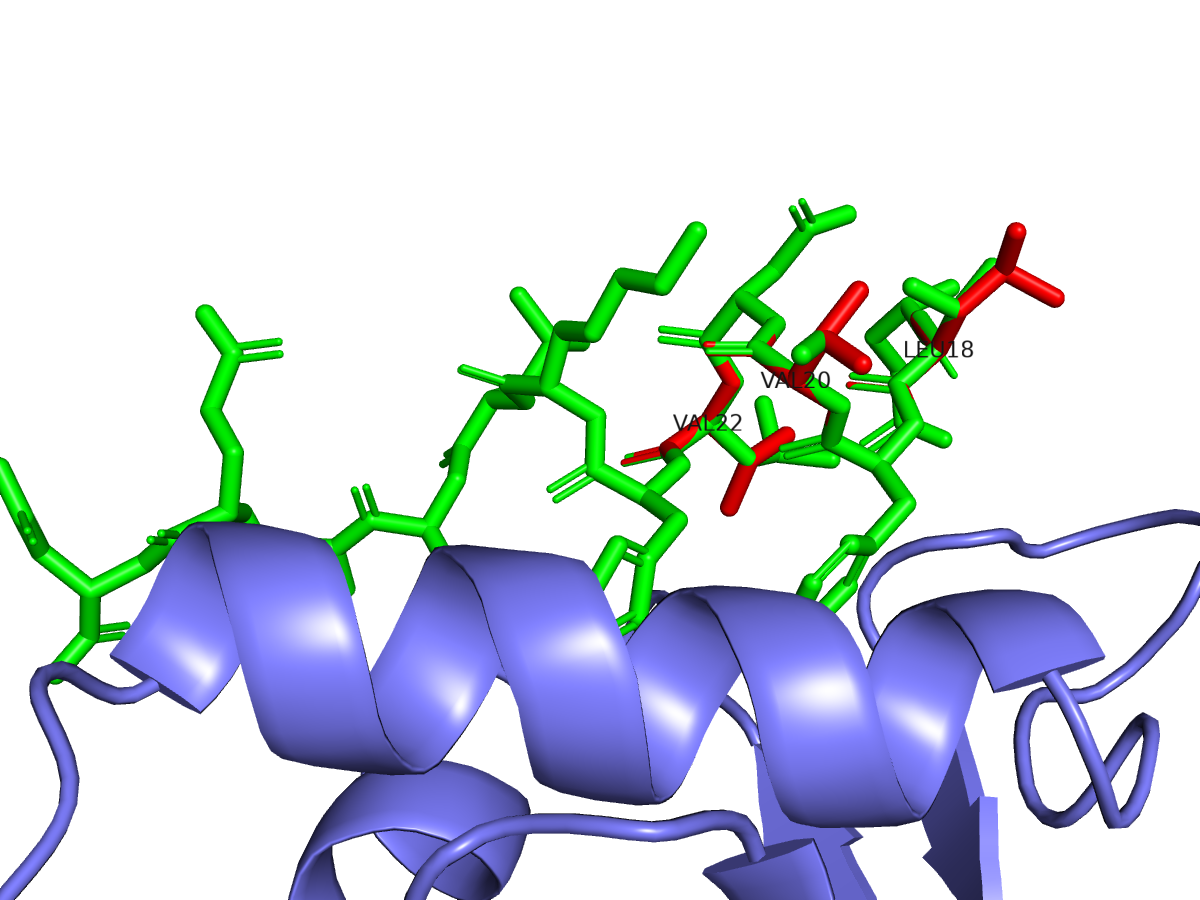
\includegraphics[width=6in]{MDM2p53_comparison_labeled.png}
\caption{PyMOL structural comparison of the native p53 peptide and the computationally designed peptide within the MDM2 binding site. MDM2 is shown as a ribbon diagram. The native p53 peptide (green) and the designed peptide (red), generated by in silico mutagenesis of the native backbone, are overlaid as stick representations. Discrepancy between the two peptides is visible at the three design positions where side chain geometry differs as a result of the substitutions introduced by the DEE pipeline.
\figcredit{Ref.~\cite{PyMOL}.}} 
\label{fig:structural_comparison}
\end{figure}

Structural comparison of the designed peptide and the native p53 fragment was performed to visualize the conformational consequences of the three substitutions introduced by the DEE pipeline. As shown in Figure~\ref{fig:structural_comparison}, the two peptides share an identical backbone conformation, as expected given that the native p53 backbone was held rigid throughout the design process. Divergence between the two structures is localized exclusively to the three design positions (THR18→LEU, SER20→VAL, and LEU22→VAL) where differences in side chain geometry are visible. The structural overlay confirms that the designed peptide maintains the overall binding pose of the native p53 fragment while introducing hydrophobic substitutions at the variable positions, consistent with the preference of the simplified scoring function for hydrophobic residues in the MDM2 pocket.

\section{Conclusion}
This project demonstrated the feasibility of computational protein design targeting the MDM2-p53 interface using a streamlined implementation of Dead-End Elimination under minimal computational constraints. Starting from the backbone of the native p53 transactivation domain peptide from PDB structure 1YCR \cite{PDB}, side-chain identities and conformations at three positions were optimized using a simplified pairwise energy function and the Goldstein DEE criterion \cite{Dahiyat}.

DEE reduced the rotamer search space from 39,304 possible combinations to just 10, before exhaustive searching identified the GMEC as LEU-VAL-VAL replacing the native THR-SER-LEU. Comparison of the designed peptide to the native p53 fragment using the simplified scoring function demonstrated that targeted mutation of select residues can improve predicted pocket complementarity even under strict computational limitations. However, independent validation using the Rosetta ref2015 energy function \cite{RosettaScoring} revealed that these gains were achieved at the cost of overall structural stability, underscoring the limitations of simplified scoring functions that optimize for a single physical property at the expense of a more complete energetic description.

Several simplifying assumptions, required to achieve computational tractability, limited the physical accuracy of this pipeline. Centroid-based side chain geometry introduced approximation error in distance calculations relative to full atomic coordinate placement. The energy function omitted explicit electrostatics, hydrogen bonding, and conformational entropy, producing a systematic bias toward hydrophobic substitutions that was exposed by Rosetta validation. Restricting design to three positions and implementing only singles DEE further limited the scope of sequence optimization. Together, these limitations illustrate why computational capacity remains a central constraint in protein design, even when combinatorial minimization algorithms such as DEE are employed to reduce the search space.

Nevertheless, this work highlights an underappreciated value of simplified computational pipelines: their role in building understanding of complex methods. While state-of-the-art protein design demands substantial resources and expertise, implementing a stripped-down version of DEE from first principles provides deep insight into the algorithmic and physical assumptions that underlie more sophisticated approaches. Future work could target the limitations identified here to produce a pipeline with greater predictive accuracy. Equally valuable, however, would be further study of how accessible, simplified implementations of complex algorithms can lower the barrier to entry in computational protein design for students and researchers alike.
\begin{thebibliography}{10}

\bibitem{Dahiyat} B. I. Dahiyat and S. L. Mayo.
\newblock De novo protein design: fully automated sequence selection.
\newblock {\em Science,} 278(5335):82--87, 1997. doi: 10.1126/science.278.5335.82.

\bibitem{PDB} RCSB Protein Data Bank.
\newblock Structure of the MDM2–p53 complex (PDB ID: 1YCR).
\newblock Available: https://www.rcsb.org/structure/1YCR.

\bibitem{RosettaScoring} Chaudhury S, Lyskov S, Gray JJ.
\newblock PyRosetta: a script-based interface for implementing molecular 
modeling algorithms using Rosetta.
\newblock {\em Bioinformatics,} 26(5):689--691, 2010.

\bibitem{PyMOL} Schrödinger, LLC.
\newblock The PyMOL Molecular Graphics System.
\newblock Available: https://pymol.org/.

\bibitem{NCBI} National Center for Biotechnology Information.
\newblock Protein Structure and Function.
\newblock Available: https://www.ncbi.nlm.nih.gov/books/NBK6130/.

\bibitem{rotamerlib} Lovell, S. C., Word, J. M., Richardson, J. S., and Richardson, D. C.
\newblock The penultimate rotamer library.
\newblock \textit{Proteins: Structure, Function, and Genetics}, 40(3), 389--408, 2000.
\newblock Available: https://doi.org/10.1002/1097-0134(20000815)40:3<389::AID-PROT50>3.0.CO;2-2

\bibitem{vdw_energy} Lennard-Jones, J. E.
\newblock On the determination of molecular fields.
\newblock {\em Proceedings of the Royal Society A,} 106(738):463--477, 1924.

\bibitem{anchor} Khoo, K. H., Verma, C. S., and Lane, D. P.
\newblock Drugging the p53 pathway: understanding the route to clinical efficacy.
\newblock \textit{Nature Reviews Drug Discovery}, 13(3), 217--236, 2014.
\newblock Available: https://pmc.ncbi.nlm.nih.gov/articles/PMC5411684/

\end{thebibliography}


\end{document}
